% \documentclass{article}
% \usepackage{graphicx} % Required for inserting images

\documentclass{report}
\usepackage{graphicx} % Required for inserting images
\graphicspath{{./images/}}

\usepackage[top=0.7in, bottom=0.7in, left=0.5in, right=0.5in]{geometry}
\usepackage{hyperref}
\usepackage{float}
\usepackage{amsmath}
\usepackage{titlesec}

\titleformat{\chapter}[display]{\normalfont\bfseries}{}{0pt}{\Huge}
\setlength{\parskip}{0pt}  % Removes extra spacing between paragraphs
\setlength{\itemsep}{0pt}
% \title{COP290 C LAB : Spreadsheet in C\\}
% \author{Aditya Narware, Rachit Bhalani, Sabhya Arora\\2023CS10805, 2023CS10961, 2023CS11177}
% \date{February 2025}



\begin{document}
\begin{titlepage}
    \centering
    Date \hfill 2 March 2025\\
    \vspace{7cm}
    {\Huge \bfseries COP290 C LAB : Spreadsheet in C\\}
    \vspace{1cm}
    
    {\Large Aditya Narware, Rachit Bhalani, Sabhya Arora\\}
    \vspace{0.2cm}
    {\large 2023CS10805, 2023CS10961, 2023CS11177\\}
    
    \vspace{1cm}
    {\large February 2025\\}
    \vspace{1cm}
    
    \textbf{Demo Video:}  
    \href{https://csciitd-my.sharepoint.com/:v:/g/personal/cs1230805_iitd_ac_in/EYdAAlpovttDqqyyG8uE8YkBuPeXcZeU0GyfI0AGxSb95Q?nav=eyJyZWZlcnJhbEluZm8iOnsicmVmZXJyYWxBcHAiOiJPbmVEcml2ZUZvckJ1c2luZXNzIiwicmVmZXJyYWxBcHBQbGF0Zm9ybSI6IldlYiIsInJlZmVycmFsTW9kZSI6InZpZXciLCJyZWZlcnJhbFZpZXciOiJNeUZpbGVzTGlua0NvcHkifX0&e=IAhGix}{Click here to watch the video}  
    
    \vspace{0.5cm}  

    \textbf{GitHub Repository:}  
    \href{https://github.com/Sabhya-Arora/COP290-C-Lab}{Click here for the source code}
    
    \vfill
\end{titlepage}

% \maketitle
% \newpage

\section*{Introduction}
This project implements a command-line spreadsheet program that manages a grid of integer-valued cells. Users can assign values directly (e.g., \texttt{A1=3}) or define formulas (e.g., \texttt{B1=A1+1}) with arithmetic operations (+, -, *, /) and integer truncation. It supports aggregate functions such as \texttt{MIN}, \texttt{MAX}, \texttt{AVG}, \texttt{SUM}, and \texttt{STDEV}, along with \texttt{SLEEP(Value)} for timed execution.\\ 
The program features seamless navigation (\texttt{w, a, s, d}, \texttt{scroll\_to <CELL>}), output control (\texttt{disable\_output}, \texttt{enable\_output}), and terminates with \texttt{q}. It ensures robust error handling by detecting invalid input, out-of-bounds operations, division by zero, and circular dependencies, marking affected cells as \texttt{ERR} and propagating errors accordingly. Dependencies are managed through an AVL tree structure, enabling optimized recalculations where only necessary updates are performed, maintaining efficiency even in complex dependency chains.

% \section{Design decisions}
% \section{Structure of program}
% \section{Challenges faced}
% \section{Testing}

\section*{Program overview}
\begin{figure}[H]
    \centering
    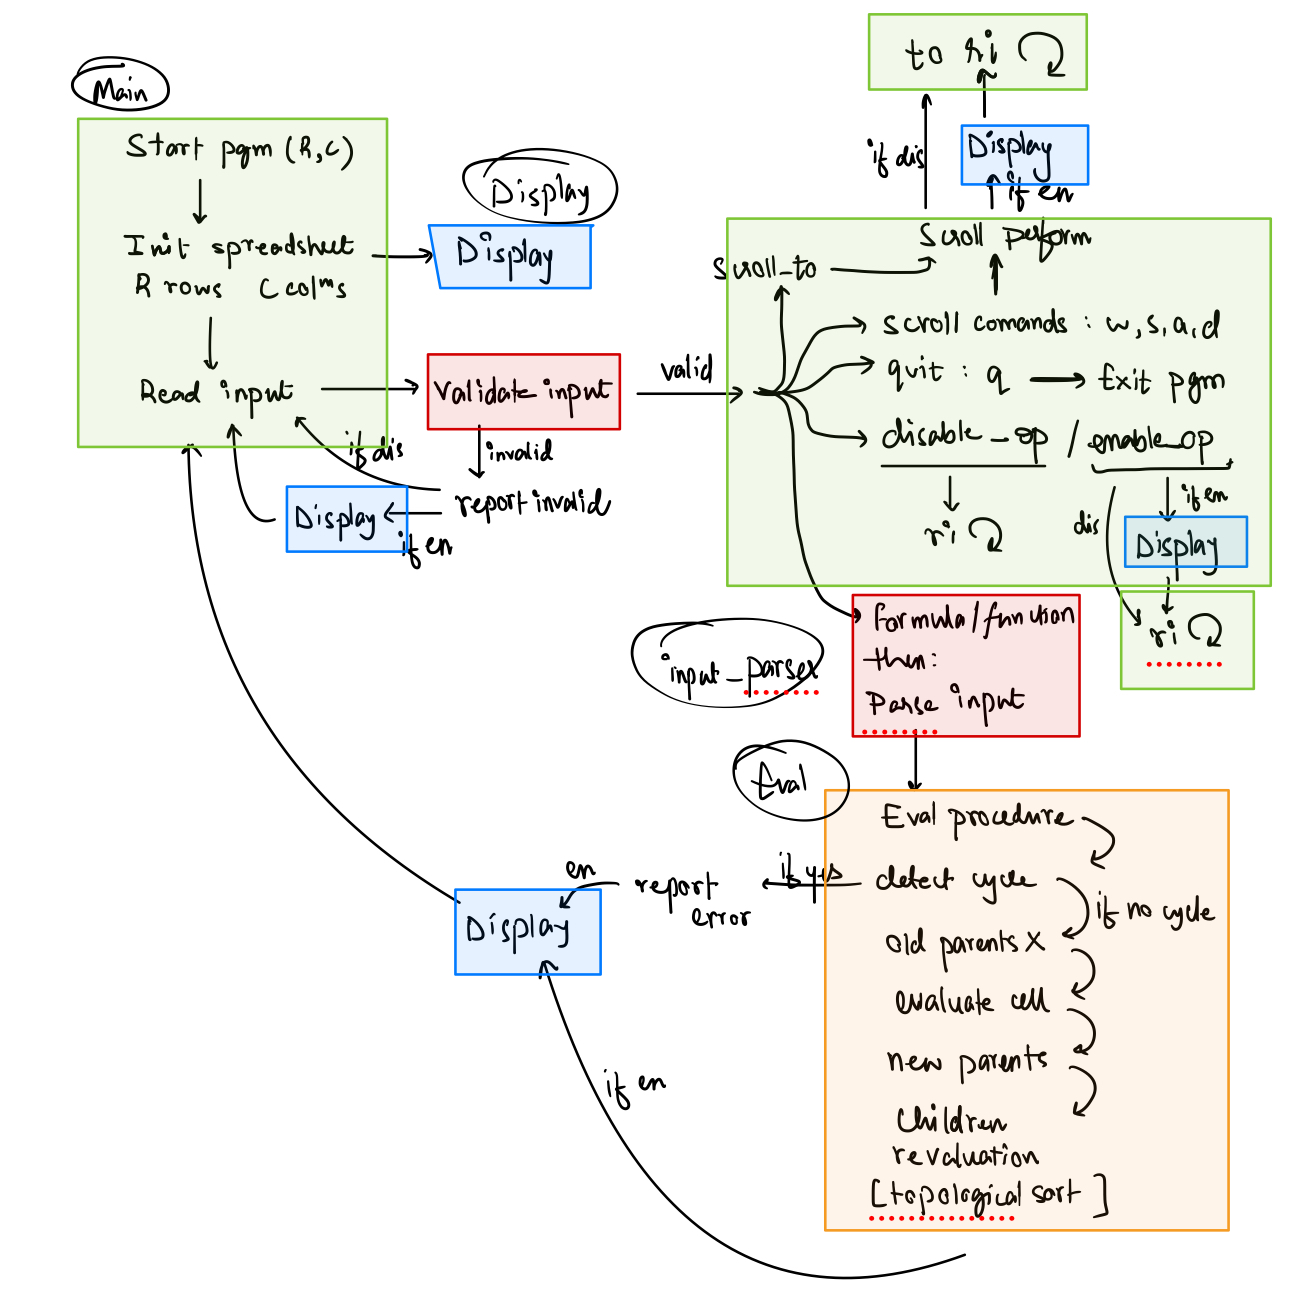
\includegraphics[width=0.7\linewidth]{figure.jpeg}
    \caption{Program flow diagram}
    \label{fig:enter-label}
\end{figure}

\section*{Main Modules}
\subsection*{Common Header: \texttt{Decl.h}}
\texttt{Decl.h} serves as a common declaration header, defining the core data structures and enumerations used in the spreadsheet program. It includes necessary library imports, macro definitions, and type declarations to facilitate consistent usage across different modules. structured approach enables efficient dependency tracking, error handling, and recalculation of affected cells.

\subsubsection*{Cell Structure Definitions}
\texttt{struct Cell}, represents an individual cell in the spreadsheet. It contains:
\begin{enumerate}
    
    \item \texttt{row}, \texttt{col}: Identifies the position of the cell in the grid.
    \item \texttt{value}: Stores the integer value of the cell.
    \item \texttt{operation}: Specifies the operation used to compute the cell’s value.
    \item \texttt{num\_parents}: Tracks dependencies, i.e., the number of parent cells influencing this cell.
    \item \texttt{associated\_const}, \texttt{associated\_sum}, \texttt{associated\_n}: Variables used for functions like SUM, AVG, and constants in arithmetic operations.
    \item \texttt{is\_faulty}: Boolean flag indicating whether the cell contains an error (e.g., division by zero).
    \item \texttt{par1}, \texttt{par2}: Pointers to up to two parent cells in binary operations.
    \item \texttt{children}: Pointer to a \textbf{LINKED LIST} tracking dependent cells that require recalculations when this cell changes.
\end{enumerate}

\subsubsection*{Operation Enumeration}
The \texttt{enum ops} enumeration defines operation types that a cell can store:
\begin{itemize}
    \item Basic operations: \texttt{CONST}, \texttt{SINGLE\_CELL}, arithmetic operations like \texttt{CELL\_ADD\_CONST}, \texttt{CELL\_MULT\_CELL}, etc.
    \item Aggregate functions: \texttt{MIN}, \texttt{MAX}, \texttt{SUM}, \texttt{AVG}, \texttt{STD\_DEV}.
    \item Special operations: \texttt{SLEEP\_CONST}, \texttt{SLEEP\_CELL}, scrolling commands (\texttt{SCROLL}), and error state (\texttt{ERR}).
\end{itemize}



\subsection*{Input Parsing: \texttt{input\_parser.c}}
\subsubsection*{Validity Checker}
The validity checker processes the input string by converting it to uppercase and removing all spaces. This design decision ensures that input commands are case- and whitespace-insensitive. The processed string is then verified against predefined valid input formats using string operations. The checker determines whether the input conforms to any recognized command structure and the cells refer to available indices in the spreadsheet. Below is a list of all valid input formats:
\begin{enumerate}
    \item functions : \texttt{<CELL> = (one of MIN, MAX, STDEV, AVG, SUM) <RANGE>, SLEEP <VALUE>}
    \item formula : \texttt{<CELL> = <VALUE> <OP> <VALUE>}\\
    where \texttt{VALUE} can be cell/constant, op is any of '+', '-', '*'or '/'. The constant is a string of integers which may/may not begin with '-'. Range is of type\texttt{(<CELL>:<CELL>)}.
    \item commands : \texttt{W, S, A, D, Q}
    \item scroll : \texttt{SCROLL\_TO <CELL>}
    \item enable/disable : \texttt{DISABLE\_OUTPUT, ENABLE\_OUTPUT}
\end{enumerate}
Once an input string passes the validity check, it is processed further else \texttt{recognized cmd} is reported.\\



\subsubsection*{Valid Input Parser}
Commands such as \texttt{disable\_output}, \texttt{enable\_output}, and navigation controls (\texttt{w}, \texttt{s}, \texttt{a}, \texttt{d}) are handled directly in the main function. Other commands requiring further parsing—such as those involving mathematical operations or cell references—are processed by the parser.\\
 The parser assumes the input is valid and extracts relevant components. The main parsing function takes nine arguments: The processed input string, six \((x, y)\) coordinates representing up to three referenced cells, a single constant value, an operation code corresponding to a predefined set of operations from \texttt{decl}.

This design is based on the observation that all valid operations involve at most three referenced cells and one constant. The extracted data is then passed to the main algorithm, which processes it according to the operation type. Not all extracted values are necessarily used—only those relevant to the detected operation.

The parser first identifies the operation type and updates the extracted data accordingly. The parser separates the (LHS) to identify the target cell and extracts cells and constants from the (RHS) based on the specific operation involved.


\subsection*{Linked List and Stack Data structures : \texttt{LinkedList.c, Stack.c}}
Standard implementation of linked list data structure, which (space) efficiently stores and updates dependent cells. Previously, an AVL tree was used, but a linked list was chosen due to memory constraints. This design balances correctness and resource efficiency while dynamically handling updates. Each cell maintains a list of children, ensuring correct recalculations when values change. Operations such as insertions, deletions, and traversals are optimized for minimal overhead, prioritizing space efficiency.
Stack is used for Recursion.

\subsection*{Evaluation Algorithm: \texttt{Eval.c}}
For commands such as output control and scrolling, no cell evaluation is required. However, for formula and function inputs, where a cell's value must be computed based on parsed data and its dependencies, the main evaluation algorithm manages the process. Additionally, any necessary recalculations due to dependency changes are handled within this framework.

The core steps of the evaluation algorithm are as follows:

\begin{enumerate}
    \item 	\textbf{Establishing Parent-Child Relationships:} When a formula is assigned to a cell, it (is set to) becomes a child of the cells it references. This relationship is (supposed to be) maintained within a Linked List of child nodes, as defined in the \texttt{Cell} structure.
    
    \item 	\textbf{Cycle Detection:} Before applying the new formula, the algorithm verifies that no cyclic dependency is introduced. This is achieved by ensuring that the newly assigned parent cells are not successors of the child (LHS of the input formula). A standard depth-first search (DFS) is used for cycle detection, where the old parents are temporarily marked to prevent false positives during traversal.
    
    \item 	\textbf{Updating Dependencies:} If no cycle is detected, the cell is detached from its old parents' linked lists, effectively removing its previous dependencies. Its value and attributes are then updated according to the new formula.
    
    \item 	\textbf{Appending to New Parents:} The new parent cells append this child to their respective linked lists, ensuring that the dependency structure remains well-balanced for efficient recalculations.
    
    \item 	\textbf{Recalculation Using Topological Sorting:} To ensure correctness and efficiency, the recalculations propagate depth-wise using a topological sort. This prevents redundant computations by ensuring that each dependent cell is updated only after all its required dependencies have been processed.
\end{enumerate}

The linked list structure for children ensures efficient insertions, deletions, and lookups, enabling space efficient recalculations (not as fast as AVL trees but that benefit was marginal within the memory constrains) and maintaining the integrity of spreadsheet formulas.

\subsection*{Display handling : \texttt{display.c}}
\subsubsection*{Viewport Constraints}
The program displays only a \(10 \times 10\) section of the spreadsheet at any given time. The printer function takes a starting cell (top-left corner) as input and prints the \(10 \times 10\) portion beginning from that cell provided the limits are not exceeded. 

\subsubsection*{Handling Edge Cases}
If the end row or column exceeds the maximum limits of the spreadsheet, the display adjusts dynamically to print only up to the available boundaries. The function also receives the spreadsheet’s maximum row and column indices as arguments to ensure it does not attempt to access out-of-bounds cells.


\subsection*{Main function : \texttt{C\_lab.c}}
The main function serves as the core execution loop of the spreadsheet program. It begins by initializing an empty sheet with all entries set to zero, based on the dimensions provided as arguments to the program.

Each input string is processed through the following steps:
\begin{enumerate}
    \item The input is first passed to the validator to check for correctness.
    \item If valid, the program immediately executes commands such as \texttt{disable\_output}, \texttt{enable\_output}, and scrolling commands directly within the main function.
    \item For all other operations, the input parser extracts relevant data and passes it to the evaluation algorithm.
    \item The evaluator processes the operation, updates the relevant cells, and returns the modified data.
    \item The updated spreadsheet is displayed after processing each command.
    \item If an invalid command is detected, an error message (\texttt{unrecognized cmd}) is displayed, but the spreadsheet is still printed to maintain continuity.
    \item The loop continues until the user enters the quit command (\texttt{q}), at which point the program terminates.
\end{enumerate}

\subsection*{Makefile}
Finally a make file to support make ommads for smooth execution of the porject. RThis supports:
\begin{enumerate}
    \item make : to compile the program
    \item ./target/release/spreadsheet \texttt{<arg R> <arg C>} : to initialise a spreadsheet of size RxC
    \item make report : to compile the \texttt{report.tex} and create \texttt{report.pdf}
    \item make clean : to cleanup the executables
\end{enumerate}

\section*{Edge Cases and Error Handling}
\begin{enumerate}
    \item 	\textbf{Division by Zero:} If a formula of the form \texttt{<CELL1> = <VALUE1> / <VALUE2 = 0>} is encountered, since division by zero is undefined, \texttt{CELL1} is marked as \texttt{ERR}. Furthermore, all dependent cells are updated to \texttt{ERR} recursively. If the erroneous value is later corrected, dependencies are also updated accordingly.
    
    \item 	\textbf{Unrecognized Commands:} If the input string fails validation, the program replaces the \texttt{OK} marker with \texttt{Unrecognized cmd}, retaining the previous sheet state to avoid unintended modifications. This includes cases such as referencing out-of-bounds cells, invalid range specifications, or incorrect syntax.
    
    \item 	\textbf{Cyclic Dependencies:} If a new formula introduces a cycle between dependent cells, the evaluation step detects this immediately. The program reports \texttt{Cyclic dependency} instead of \texttt{OK} and discards the invalid operation to prevent infinite loops.
    
    \item 	\textbf{Scrolling Behavior:} When reaching the boundary of the sheet, any further scrolling attempts using \texttt{w, s, a, d} are ignored, keeping the display at the last possible position without errors. If \texttt{scroll\_to <CELL>} is used and fewer than 10 rows or columns remain, it simply displays up to the available boundary without disrupting functionality. All correctness checks for scrolling are handled during parsing.
\end{enumerate}


\section*{Challenges Faced and Optimization Scope}
\begin{enumerate}
    \item 	\textbf{Memory Constraints:} Given the potential spreadsheet size (up to $999 \times 18278$), memory usage escalates rapidly. In extreme cases, operations affecting all cells can consume several gigabytes within a few commands. While AVL trees provide efficient lookup times, they were replaced with linked lists to prioritize space optimization, which proved more practical for real-world use cases.
    
    \item 	\textbf{Input Parsing:} Converting raw input strings into structured commands required robust validation and parsing. The validator discards malformed inputs, while the parser extracts relevant data for evaluation, ensuring seamless communication between modules.
    
    \item 	\textbf{Design Considerations:} Ambiguities in command behavior, such as scrolling past boundaries and handling prefixed operators, were resolved with practical constraints. The final design ensures scrolling remains within bounds and allows only a leading minus sign before constants for simplicity.
    
    \item 	\textbf{Testing Strategy:} Given the complexity of multiple interdependent modules, a systematic testing approach was adopted. Core functions were validated using focused test cases, with special emphasis on the validator and parser due to the diverse range of possible errors. For large-scale tests, output was disabled during execution and enabled only upon completion to conserve memory.
\end{enumerate}

\end{document}